% !Mode:: "TeX:UTF-8"
\chapter{分支预测器介绍}


本章首先介绍香山处理器第二版分支预测的整体架构,各个预测器在流水级中的先后关系和联系。其次针对每个预测器都介绍了它们的预测原理和功能。并指出它们相对于第一版设计做出的修改,以及做出相关修改的原因。

\section{分支预测整体结构}

香山第二版分支预测架构采用的是4级流水设计,架构图如图\ref{fig:figure21}所示。参考了BOOM提出的COBRA架构\cite{cobra},能够更加灵活的管理和组织预测器。在4个流水级中,S0主要负责收集S1、S2、S3流水级的预测结果,以及取指单元 (Instruction Fetch Unit, IFU)和流水线后端 (Backend) 发回的分支误预测信息,从中选择出下一周期需要进行预测的指令pc (Program Countet),即指令在其内存中的地址。然后将该pc以及其他用于预测的信息发给各个预测器,不同的预测器得出预测结果的时间需要1到2周期不等。

\begin{figure}[htb]
	\centering
	\setlength\tabcolsep{3pt}  % 同一行中的图片间隔
	\vspace{5pt} % 图片上部的空白,如果太小的话,图片顶部会与正文内容十分接近
	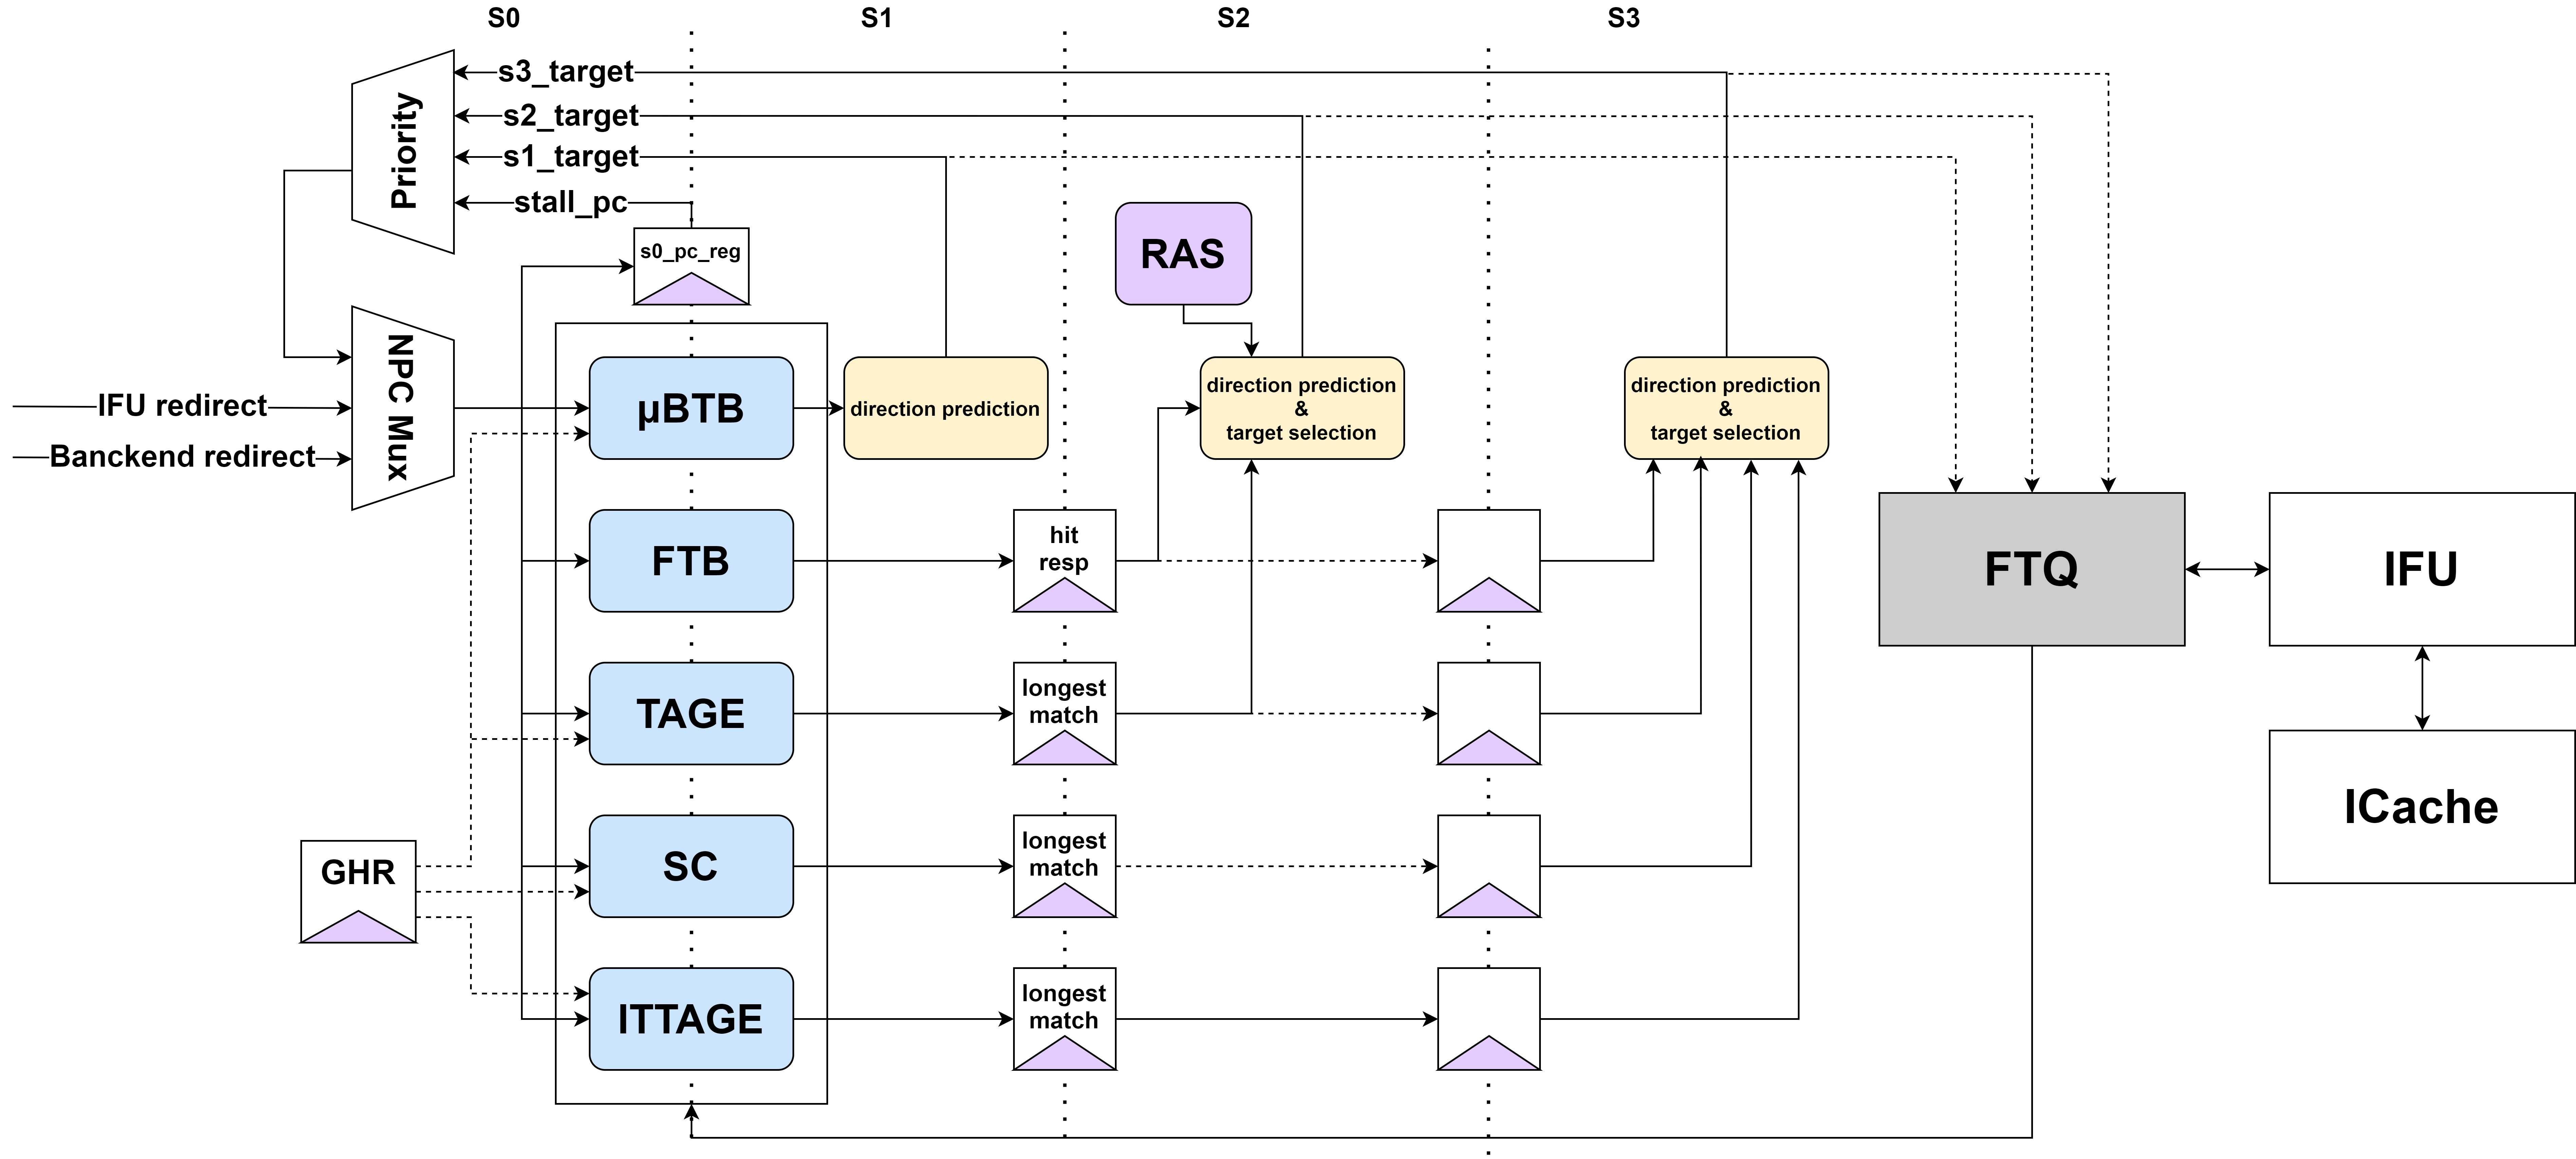
\includegraphics[width=1\textwidth]{BPU-FTQ-IFU.jpg}
	\caption{香山处理器第二版分支预测架构图}
	\label{fig:figure21}
\end{figure}

香山分支预测的主要预测器使用的是TAGE算法\cite{tage, tage-sc-l, new-case-tage},但是由于TAGE预测算法需要索引预测表,还要计算哪些表命中,最后从中选择出历史长度最长的表得出预测结果,逻辑比较复杂,需要的时间更长,超过了一个周期所需的时间。如果只使用TAGE进行预测的话,那么分支预测每2个周期才能够发出一个取指请求,显然破坏了流水线,因此为了能够让分支预测流水线无气泡的流水,需要一个逻辑比较简单,每周期都能够做出一次预测结果的预测器,也就是负责在S1做出预测的Micro BTB,它每周期都能够针对上一个周期的pc给出预测结果,及时的给出下一周期需要预测的pc,这样就能够让流水线无气泡的工作。之后S2能够得到由FTB、TAGE和RAS联合做出的预测结果,由于S2的算法更复杂,能够覆盖更多的情况,因此可以认为它的预测准确率高于S1。当出现S2的预测跳转方向和跳转目标地址和S1预测的结果不相同时,以S2的预测结果为准,这意味着之前S1预测的结果需要修正,需要清空S2之前的流水线,从S2预测的下一周期目标地址开始重新预测,这时分支预测流水线就会产生1拍的气泡。同样的,在S3会使用SC和ITTAGE再进行一次预测, 一般来说认为这次的预测是最准确的,也就是说S2的预测结果和S3预测结果不同时以S3的结果为准。当出现S2和S3预测结果不同时,也需要刷新分支预测流水线重新取指,这会带来2周期的气泡。

分支预测还需要管理分支历史,由于使用了Fetch Block作为基本分支预测单位,而Fetch Block中的特性使得在更新分支历史时有些许的不同。这部分会在第四章中详细说明。

相比于第一版的设计,第二版最重要的改动就是限制分支预测宽度和将取指功能和分支预测部分解耦,将分支预测流水线和取指流水线统一称为前端流水线,而在这之后的流水线称为后端流水线。通过重构前端,将取指单元的执行顺序移到了分支预测之后,这样做的好处在于可以减少一些前端流水线的气泡。

\section{Composer设计介绍}

参考了BOOM提出的COBRA架构,因此第二版架构中所有的预测器都继承自同一个BasePredictor基类,它们有着统一的接口,在实例化预测器时,所有的预测器都按照优先级顺序排列存储在一个components列表中。所有的预测器之间的连线和数据传输都由Composer模块负责。

除了负责连线以外,Composer模块另一个重要的作用就是为所有预测器的meta信息进行打包和解包。由于分支预测在运行时,会产生许多的预测信息,有些预测信息需要保存起来,在指令提交时取回这些信息用于恢复和训练分支预测器,这类信息统称为meta信息。而不同预测器的meta信息数量类型都不相同,为了便于存储,将每一次预测中所有预测器的meta信息都强制转换为无符号整数类型,将它们按照预测器优先级顺序拼接起来,变成一个超长的无符号整数类型,这样既方便了存储,也提高了代码的可读性。当指令提交或误预测时,再把meta信息取回,按照之前打包时的顺序,将所有的meta信息拆分开,再转为各个预测器所需要的meta信息类型,分配给各个预测器。这部分工作就是由Composer完成的。

通过使用Composer组织所有的预测器,在需要增加或减少预测器时,由于接口都是统一的,就可以免去预测器之间复杂的连线操作,极大提升了开发效率,也降低了出错的可能。虽然所有的预测器都使用统一的接口,那么对于每个预测器来说,必然有些接口是冗余无用的,但是由于Chisel的语言特性,这些没有在预测器中使用的接口,编译成Verilog代码时都会被编译程序自动优化掉,因此在生成的Verilog代码中,所有的预测器都有着自己独有的接口,不会存在冗余的情况。

\section{FTB设计介绍}

由于分支预测通常运行在取指之前,因此无法通过对指令码进行预译码来识别一条指令是否是分支指令,也无法知道一条分支指令的跳转目标地址。即使在第一版的设计中,取指和分支预测同时进行,等到将指令码从指令缓存 (Instruction Cache) 中取回时,也要等到2周期以后。由于局部性原理,执行过的分支在之后再次被执行的可能性很大,因此需要在程序执行过程中,将已经执行完毕,知道分支类型、跳转目标地址等相关信息的分支指令都保存在一个buffer中,通过它们的pc进行索引,这样下次再遇到同一条分支指令时,就可以通过查找这个buffer来获得它的相关信息,从而得知它的指令类型和跳转目标地址。这就是BTB (Branch Target Buffer) 的主要功能。它负责在预测时指出哪些指令是分支指令,以及它们对应的跳转目标地址。

在第一版设计中的BTB,以单条分支指令为基本单位,而由于前端的取指宽度是32Byte,算上4Byte长的普通指令和2Byte的压缩指令,一次取指中最多可能同时有16条分支,即16条都是压缩指令的情况,因此第一版设计中的BTB总共有16个bank,每个bank对应指令块中可能是一条分支指令的起始位置。而相对的进行分支预测时,也要同时对这16条指令进行索引和预测,再最后要从这16条预测结果中选出最终生效的一条指令,将其预测的下一周期取指pc送回S0。

在第二版的设计中,为了减少分支预测宽度,降低流水级中的逻辑门级数,采用了Glenn提出的FTB (Fetch Target Buffer) 设计\cite{scalable-frontend},相比于BTB,FTB主要的改变在于将buffer中储存的项由单条分支修改为了一个有一定约束的取指块 (Fetch Block),通过给定的约束,前端每次的取指宽度由32Byte的固定大小改为了不固定的大小,每个Fetch Block的大小由block中分支指令的分布决定,Fetch Block限制了每个block中分支指令的数量上限,在第二版设计中,限制每个block中最多只能够有2条条件跳转指令 (branch)和一条无条件跳转指令 (jump)。通过这种设计,能够将分支预测的宽度由第一版的16降低为2,从而减少最后的选择逻辑门级数,达到减少组合逻辑电路延迟的效果。在第三章中会更加详细的讨论FTB的实现。

第一版设计中,BTB总共有2K项,16个bank,2路组相联。第二版中FTB虽然也有2K个项,4路组相联,但是由于一个FTB表项所占的空间几乎等于原来BTB一个表项的2倍,因此实际上第二版实现FTB所使用的SRAM大小应该是翻倍了的,这会带来一定的性能提升,同时会增大分支预测部分的面积。

\section{Micro BTB设计介绍}

Micro BTB作为一个小型的预测器,需要在每周期内都得出一个初步的预测结果,来保证分支预测流水线的连续。因此首先具有一个小型FTB的功能,它也能够保存分支指令的信息,但是由于它需要在很快的时间内做出一个初步的预测,因此它的逻辑必须简单,使用的硬件资源必须足够小,因为过于复杂的逻辑和过多的面积都会导致它无法按时给出预测结果。

在第一版的设计中,Micro BTB就是一个小型的BTB,并且自带了一组两位饱和计数器,有16个bank,每个bank中可以存储16条分支指令的信息,按照全相联存储。在预测时通过索引分支指令信息,并且以两位饱和计数器的值来给出预测结果。由于存储的信息很少加上预测算法简单,因此Micro BTB的预测速度非常快,当拍就可以给出预测的结果。

在第二版的设计中,由于需要满足更高的频率要求,Micro 由原来的全相联修改为了256项直接映射,使用SRAM实现。直接映射在索引和判断命中时能够有更短的电路延迟,且使用单口的SRAM在面积上也不会比第一版的寄存器堆大太多。另外去除了原来的两位饱和计数器组,修改了Micro BTB的预测算法,首先使用要预测的pc和全局历史哈希做索引,当Micro BTB命中,即发现当前pc对应的取指块已经被保存时,它会依据上一次索引到该项的分支的跳转方向,以此作为这次的预测结果。这种逻辑会比更新和计算饱和计数器更加简单,同时不会有太大的性能损失。

\section{RAS设计介绍}

RAS (Return Address Stack) 是一个专门针对call和return指令优化的预测器。知道在程序中往往存在着大量的函数,它们会不断地调用和返回,指令执行过程如图\ref{fig:figure22}所示,通常程序执行某个函数时,首先会使用一条call指令跳转到函数的起始地址,然后从起始地址顺序往下执行,当函数执行完后,最后会有一条return指令,再将程序跳转回call指令之后的下一条指令继续执行。当然在执行函数的过程中也有可能继续调用一个新的函数。由于函数调用是递归的,因此可以使用一个栈结构来保存所有函数调用的返回地址。当检测到一条call指令时,将这条call指令之后的下一条指令存入RAS,然后当检测到一条return指令时,就将RAS栈顶保存的地址出栈,作为这条return指令的跳转目标地址。

\begin{figure}[htb]
	\centering
	\setlength\tabcolsep{3pt}  % 同一行中的图片间隔
	\vspace{5pt} % 图片上部的空白,如果太小的话,图片顶部会与正文内容十分接近
	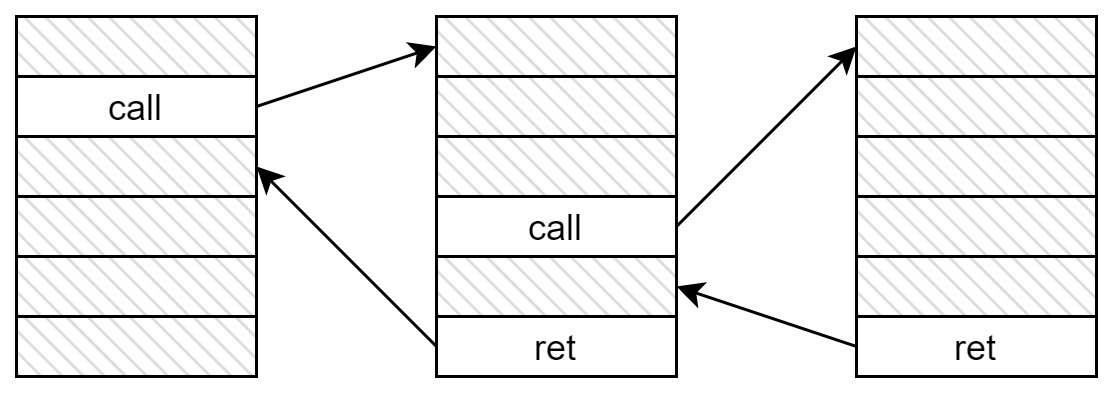
\includegraphics[width=0.8\textwidth]{function-call-ret.jpg}
	\caption{在程序中函数的调用和返回}
	\label{fig:figure22}
\end{figure}

由于程序中有大量的类似于递归调用的行为,即有的函数在满足条件时,会不断地自己调用自己,在这种情况下,每次要保存的返回地址起始都是相同的。因此每个RAS项都带有一个计数器,当这一次调用的返回地址与栈顶元素的返回地址相同时,就不会将这次调用入栈,而是给栈顶元素的计数器加1。同样的在return指令时,首先会检测栈顶元素的计数器,如果计数器大于1,则不弹出栈顶元素,只是将栈顶元素的计数器减1,直到计数器为1时才出栈。

这样修改能够减少RAS在遇到某些特别深的递归时,不至于一直入栈相同的返回地址,导致栈溢出,能够提高RAS的预测准确率。

而为了减少预测时读取RAS的延迟,另外使用了一个专门的寄存器用来存储当前栈顶的地址副本,在每次RAS入栈出栈时也会同时维护这个副本。当检测到一条return指令时,就可以直接使用这个单独的寄存器,而不用从整个RAS栈中读取栈顶元素,能够节省从RAS栈中索引出栈顶元素所需要的时间。

RAS在分支指令出现误预测时需要恢复,不然可能会出现地址错乱的情况,RAS在误预测时修复的方法有很多种\cite{ras-recovey, ras-revisited},而第二版实现时使用了一种较为简单的恢复方法,即在分支预测时将当前的栈顶指针和栈顶元素保存起来,在恢复时只恢复栈顶元素和指针,这样一来既能够简化恢复逻辑,也不会带来过多的误预测。

\section{TAGE设计介绍}

TAGE (TAgged GEometric history length branhc predictor) 是由André提出的一种预测器\cite{tage},曾经多次夺得过分支预测大赛 (CBP, Championship Branch Prediction) 的冠军,之后由许多研究者对其不断地优化和改进,是目前公开的分支预测性能最好的预测器之一。TAGE是一个使用全局历史索引的方向预测器,也就是说它只会用来预测分支是否跳转,而跳转目标地址需要由FTB、RAS或ITTAGE来提供。


\begin{figure}[htb]
	\centering
	\setlength\tabcolsep{3pt}  % 同一行中的图片间隔
	\vspace{5pt} % 图片上部的空白,如果太小的话,图片顶部会与正文内容十分接近
	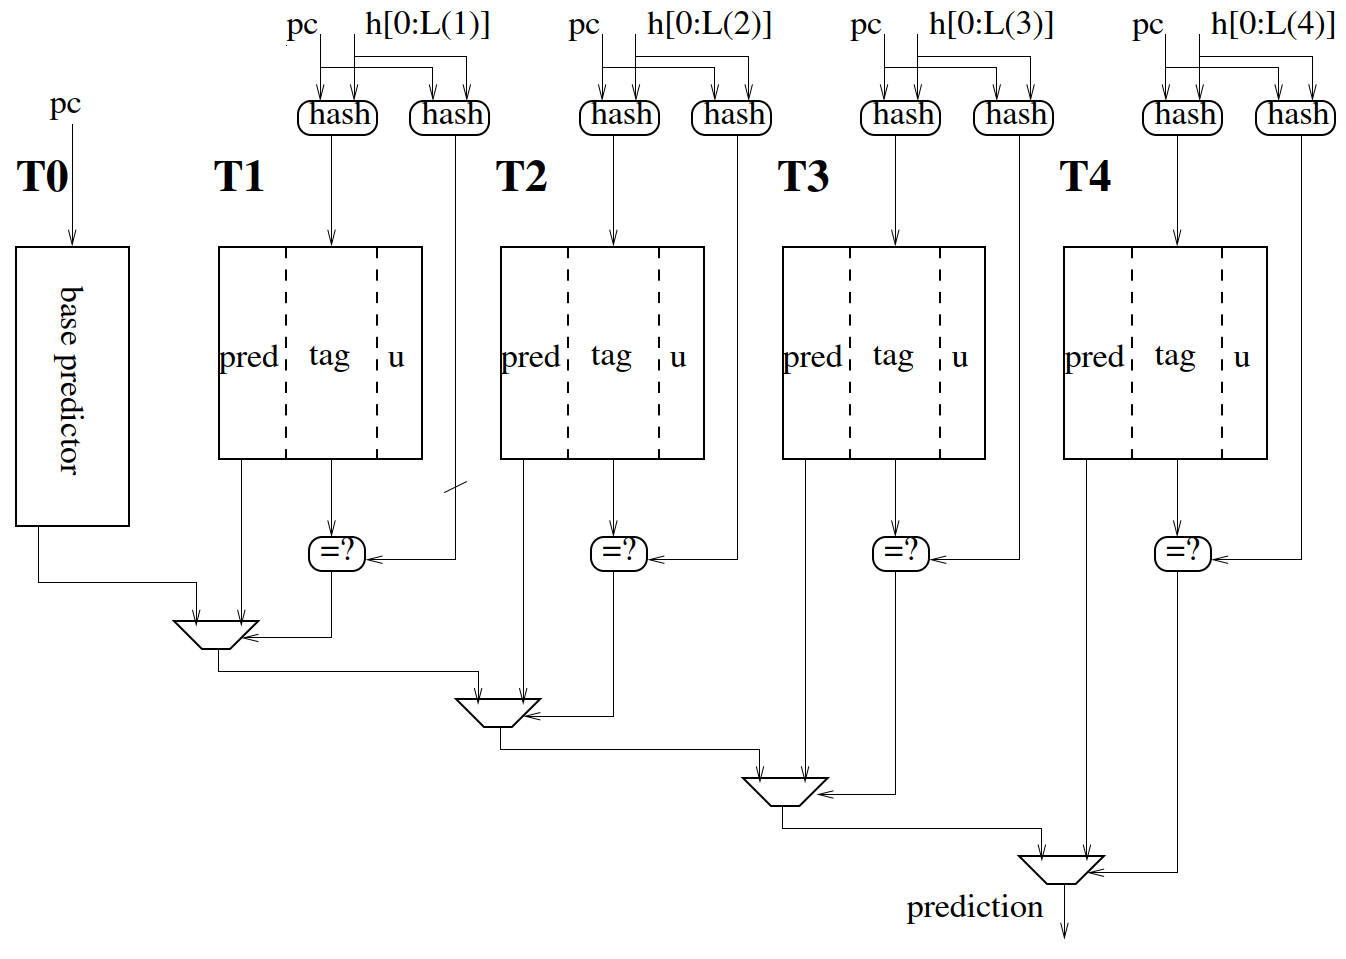
\includegraphics[width=1\textwidth]{tage.jpg}
	\caption{TAGE预测器结构图\cite{tage}}
	\label{fig:figure23}
\end{figure}

TAGE预测器由一个基本表T0,和n张预测表Ti (i=1,2,3,...,n) 组成,其中基本表是一组使用SRAM存储的2位饱和计数器。而每张预测表的单个表项中都有一个valid位,一个tag,以及一个3位饱和计数器。每张表的大小,用于索引的折叠历史长度,以及tag长度都是可配的,通常来说从T1到Tn,用于索引的折叠历史长度程几何递增关系。第二版的TAGE表配置如表\ref{tb:table21}所示。

\begin{table}[]
	\caption{香山第二版分支预测架构TAGE预测表配置}
	\label{tb:table21}
	\centering
	\begin{tabular}{|c|c|c|}
		\hline
		项数   & 历史长度   & tag长度   \\ \hline
		4096 & 8 & 8 \\ \hline
		4096 & 13 & 8 \\ \hline
		4096 & 32 & 8 \\ \hline
		4096 & 119 & 8 \\ \hline
	\end{tabular}
\end{table}

在使用TAGE做预测时,需要知道待预测指令的pc,以及当前的分支全局历史,由于全局分支历史是一个较长的bit串,所以先使用简单的哈希算法将其折叠,然后再与pc一起计算出一个值,使用这个值去索引预测表,由于不同的预测表使用的折叠历史长度不同,因此相同的pc和全局历史在不同的预测表中也会映射到不同的表项中。

在索引到每张预测表中的表项后,首先会检查这个表项是否valid,如果是valid,那么继续比对其中存储的tag与pc是否匹配,如果匹配了则代表这张表命中了,选择该表项的饱和计数器作为这张预测表的预测结果。在多张预测表命中时,TAGE会选取折叠历史长度最长的那张表的预测结果,作为整个预测器的预测结果,这个表成为provider。而如果T1到Tn都没有命中,则会使用T0基本表中的饱和计数器作为预测结果。

而如果发现provider中的表项是新写入的,其中的值还是写入时的初始值,可以认为这个表项是还没有训练完成的,因此TAGE在查找所有命中的表中最长历史的表时,也会同时查找第二长历史的表,称为alrProvider如果发现匹配的最长历史表中的计数器是初始值的话,就会使用匹配的第二长历史表的预测结果。

但是为了优化时序,减少路径延迟,在第二版的设计中一律将altProvider设为T0的预测结果。

% 更新逻辑

在有分支指令从后端发来更新时,首先需要检查之前这条分支预测时是否有预测表命中,如果有命中的表,就会更新对应的表中的表项里的饱和计数器,如果分支跳转则饱和计数器加1,不跳转则饱和计数器减1。

% 分配新项
当一条分支发来更新时,如果它命中的表Ti不是Tn,则会去选择一张表Tj (i<j<=n),且u标志位为false的项分配,从Ti+1到Tn查找,选择第一张符合要求的表进行分配,新分配的表项的饱和计数器根据这条分支的跳转方向来决定,如果跳转则置为weak taken,否则置为weak untaken。

u标志位用于在分配新的表项时来决定分配给哪一张表,u位在一条分支指令最终预测正确,但是它的altProvider预测结果是错误时增加,当所有的u都为true时,还有新的项要写入,则复位计数器tick递增,否则递减,当到达一定的值时,就会把所有的u都复位。

由于在一条分支指令从预测到更新之间有一定的延迟,而这段时间内这条分支对应的表项有可能会有其他的写入,因此在实现时借鉴了BOOM中的wrbypass技术,通过一个简单的buffer,记录最近的TAGE写入,这样在更新饱和计数器时,首先去查找wrbypass中有没有对应的表项,如果有,就以wrbypass中存储的饱和计数器为基础去更新,如果没有就使用从后端传回来的meta信息中的饱和计数器去更新。

在第一版的设计中TAGE的基本表直接复用了BIM (Bi-Model Predictor),而在第二版中为TAGE添加了单独的基本表,主要原因是在第二版的设计中S2就能够得到TAGE的预测结果,因此,不需要BIM。其次就是TAGE的基本表的更新策略和BIM有些许的不同。

% TAGE由多张预测表组成,每张表通过不同长度的分支历史来索引,表中的每一项都是一个饱和计数器。每次预测时会同时查找所有的表,然后从中选择出历史长度最长且tag匹配的表,以它的饱和计数器值作为分支预测的结果。

\section{SC设计介绍}

SC (statistical corrector) 是TAGE预测器的一个组件,如图\ref{fig:figure24}所示。主要针对的是对某个方向只有很小的偏差,但是与历史路径相关性不强的分支\cite{tage-sc-l, isl-tage}。这种类型的分支有时TAGE无法准确预测。

SC也是由几张表组成的,每张表中的表项有2个6位的计数器,一个用于在TAGE预测跳转时使用,一个用于TAGE预测不跳转时使用。在预测时会根据带预测指令的pc和折叠历史进行哈希索引。将每张表索引出来的计数器的值相加,再加上TAGE预测的结果。然后使用最终的和与某个动态变动的阈值进行比较,再通过TAGE的预测结果进行一个二选一,得出最后的预测结果。

在预测时SC会有一个动态的阈值,这个阈值会动态的改变,每次会根据待预测指令的pc和历史索引每个表,将得到的结果相加,当相加的结果大于阈值时就翻转TAGE的预测结果。

Threshold自身有一个5位的计数器,每次有指令更新时,如果SC曾经做出过预测,且满足一定条件时进行更新。而阈值也会根据新更新的计数器计算,如果饱和计数器达到最大值,且当前的threshold小于最大值,则增加;当饱和计数器达到最小值,且当前的threshold大于最小值,则减少。

% 每次预测时SC会收到待预测指令的pc,分支历史,以及TAGE做出的预测结果。SC会索引每一张表,并取出每张表对应的两个饱和计数器,最后将它们相加,再加上TAGE的饱和计数器,得到一个totalSum。当TAGE命中且,totalSum相加大于0,且大于当前的threshold,或相加小于0,且相加小于负的threshold时,SC会做出预测,预测方向为所有SC表取出饱和计数器之和是否大于0.通过TAGE预测是否跳转来选择用0还是1。

与TAGE类似,SC也有wrbypass的结构,用来保证在指令从预测到更新期间有其他的指令更新了相同的表项,保证了用于更新的计数器是最新的值。

\begin{figure}[htb]
	\centering
	\setlength\tabcolsep{3pt}  % 同一行中的图片间隔
	\vspace{5pt} % 图片上部的空白,如果太小的话,图片顶部会与正文内容十分接近
	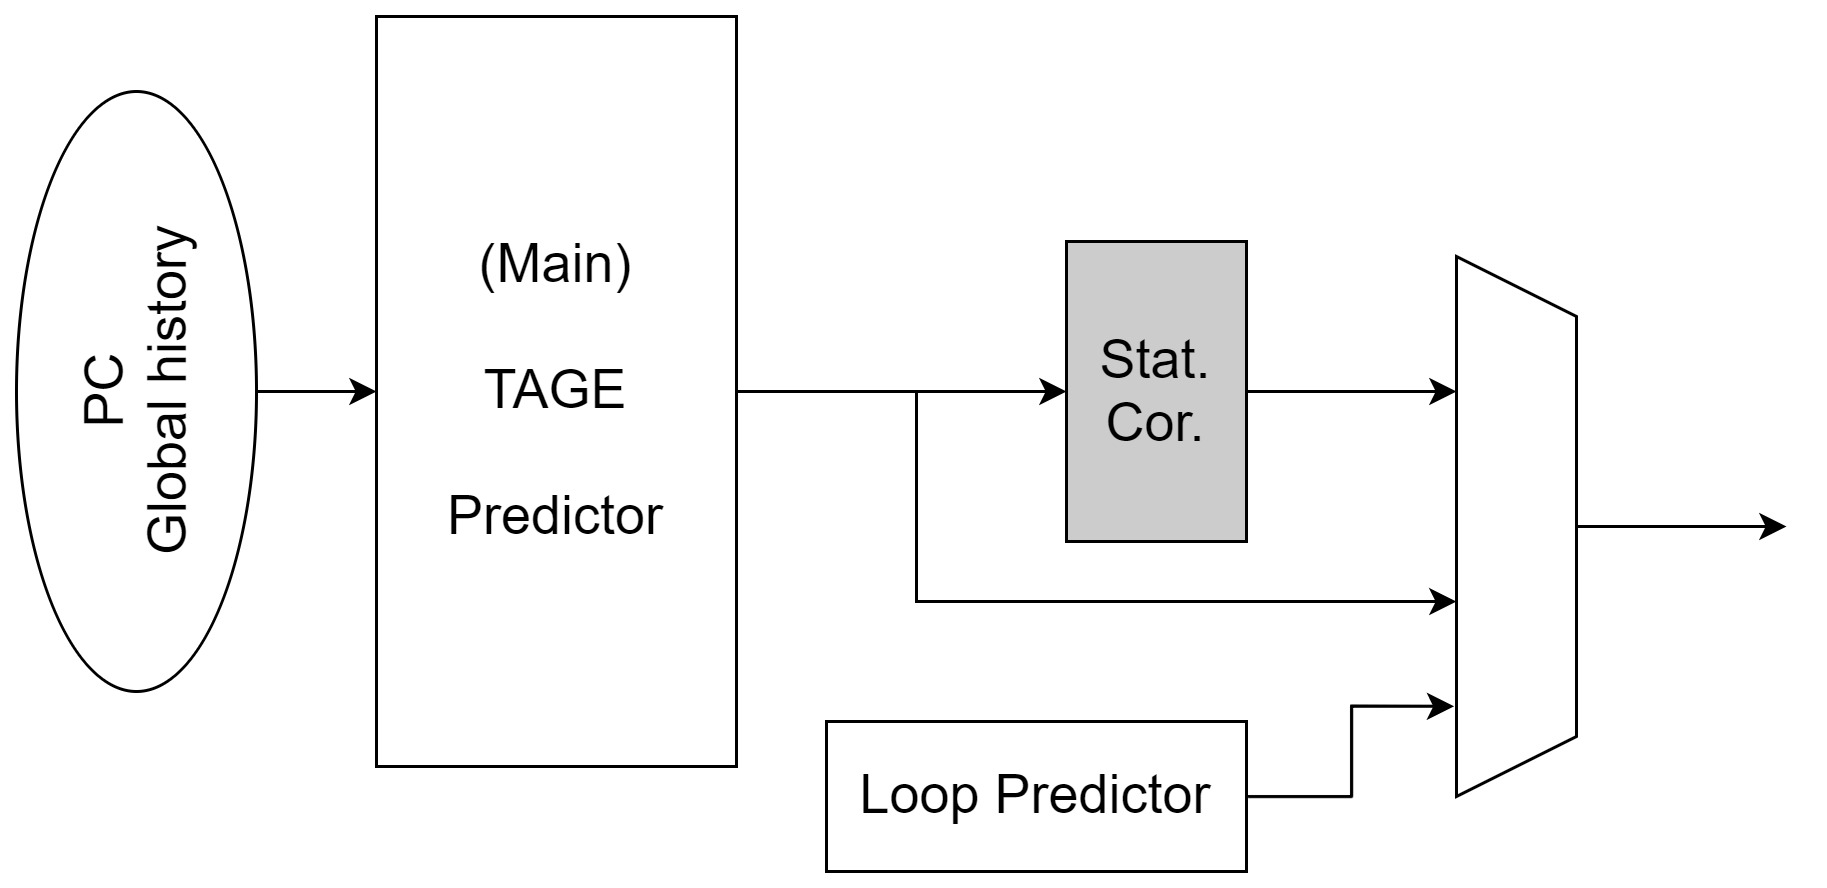
\includegraphics[width=0.8\textwidth]{sc.jpg}
	\caption{TAGE-SC-L架构图\cite{tage-sc-l}}
	\label{fig:figure24}
\end{figure}

% 还有那个算threshold的算法

\section{ITTAGE设计介绍}

ITTAGE (Indirect Target TAgged GEometric history length branhc predictor)\cite{tage, ittage} 是一个专门针对间接跳转分支的预测器,也是由André提出的,其算法大部分与TAGE相同。不同之处在于TAGE中用于判断跳转方向的饱和计数器被替换成了一个跳转目标地址和一个置信度计数器,在预测时通过pc和分支历史索引到的表项返回,如果这条分支被预测跳转,则作为这条分支的跳转目标地址。

\section{分支历史管理策略}

在分支预测中分支历史管理也是一个重要的功能。在第一版的设计中,参考了BOOM,将每个32Byte的取指block视为整体,每个block在全局分支历史中占用1bit,无论其中有多少条指令。在更新分支历史时通过寄存器移位来更新分支历史,误预测恢复时也是直接将之前保存的完整分支历史覆盖回全局历史寄存器中。

而在第二版架构中,为了令全局分支历史更加准确,改为了每一条分支指令在全局历史中占用1bit,这样的话全局分支历史的管理策略就需要做相应的改动,为此设计了新的分支历史更新逻辑,在需要更新分支历史时,需要判断当前Fetch Block中有多少条需要加入到分支历史中的分支指令。此外第二版中还将原来的寄存器移位更新改为了使用分支历史指针来管理更新,在误预测恢复时也是直接传回误预测指令所对应的分支历史指针做恢复逻辑。

在第二版的架构中除了保存完整的分支历史以外,还保存了用于索引TAGE、ITTAGE等预测器所需要的折叠分支历史,不同于第一版,每次需要使用折叠历史时都是用完整的分支历史计算,这次的这叠分支历史是直接按照折叠的状态来维护的,这样能够得到更好的时序结果。

在分支预测时,S0的分支历史会顺着流水级一级级往下传,确保每个流水级预测时使用的都是相同的分支历史,同时每个流水级也会生成根据自己本身预测结果更新过的分支历史,S0分支历史寄存器的历史会通过一个优先选择器,选择合适的新分支历史来源进行更新。

\section{本章小结}

本章首先详细介绍了本文提出的分支预测架构的流水线设计和工作流程,给出了架构图,展示了每个预测器在流水线中的不同位置。之后单独列出了Composer模块,以及FTB,Micro BTB,RAS,TAGE等预测器的功能和算法。其中主要介绍了TAGE预测器的功能逻辑,以及相对于第一版架构做出的改进。为之后两章的内容做了铺垫。